\chapter{Evaluation and Testing}\label{chp:tes}
Testing is an essential part of the project as it for allows unforeseen issues to be detected. The system will first be tested in its entirety to ensure it functions correctly, this will be done in parallel with development. Unit tests will also be written for each section to ensure the development of functioning modules. The system must also meet the requirements set out in Chapter \ref{chp:req} and as such will be tested based on these requirements. This chapter will also evaluate the final developed project both in its overall state and in its three separate parts. This chapter will also assess the limitations of the project.

\section{Full System Testing}
Full system testing involves testing the system in a use case scenario. In this case the system will be tasked with generating normal network data and network data from the attacks found in the \texttt{attacks} directory. The data is automatically processed and stored to a CSV file. 
The Full system utilises a network which resembles that of \ref{fig:vnd}. The attack machine being a Kali Linux machine and the target machine being either a Windows XP or Windows 7 machine, as the switch to windows 7 happened early on but not before some data was generated. The normal network data was generated on the Host PC connected to the network. The noise from other devices connected to the network in normal network data generation serves to help simulate the more unpredictable nature of normal network data.

Throughout development the parts of the system which were deployed were utilised to either, generate or process data to be used in the next part of the development. Because of this the full system deployment was done during the Implementation plan detailed within the Implementation chapter.

The dataset generated consisted on 20,379 rows, the dataset mainly consisted of normal network data. The normal network data was run for four hours, this was done in the hopes of reducing the number of false positives. The rest of the data was generated in different chunks between 10 minutes and 30 minutes. This dataset is utilised thought testing to train models.

This scenario is built to represent a typical usage of the tool. The model generated from this scenario will be able to detect different types of threats. The full scenario uses the attacks from Table \ref{table:attacks}:
\begin{enumerate}
    \item Generate normal data for 4 hours
    \item Generate attack data for 10 - 30 minutes
    \begin{enumerate}
        \item synflood
        \item udpflood
        \item finflood
        \item pshackflood
    \end{enumerate}
    \item Process data (done automatically in the generate command)
    \item Train model with the generated data
\end{enumerate}
Unit tests were written to test each step of the above scenario, the unit test for the normal data generation is given in Listing \ref{code:unt}:
\begin{lstlisting}[language = python, caption = Normal Data Unit Test, label=code:unt]
def test_normal_generation(self):
        """
        Test that normal data can be generated
        """

        data_generation.DataGen("normal",
                                None,
                                None,
                                10,
                                None,
                                None,
                                None,
                                None,
                                None,
                                "data.csv",
                                None)
        
        time.sleep(1)
        self.assertTrue(os.path.exists("data.csv") and os.path.getsize("data.csv") > 0)
\end{lstlisting}

These tests utilise the native \texttt{unittest} python package. The tests can be run in the command line and can be executed individually by using the \texttt{python -m unittest test\_module.TestClass.test\_method} command. These unit tests check to see if the file which is supposedly generated by the package has been generated and contains text. 

Finally a large test was written which executes the relevant commands from the command line to run the above scenario fully. The config file must be first configured and then the commands are executed sequentially. Finally culminating in the model being generated.
\subsection{Time to Generate Normal Data}
The unit test for generating normal data is used to test the speed of setting up, running and processing normal network data. The unit test was run 5 times, each time taking the time needed to run the unit test native to the \texttt{unittest}. The First unit test can be seen in Listing \ref{code:unt}, this will run Normal network generation for 10 seconds.
\begin{table}[H]
	\begin{minipage}{0.4\linewidth}
        \centering
        \caption{Results of Unit Test 1}
        \label{table:unittest1}
        \begin{tabular}{cc}
         \textbf{Test No.}&\textbf{Time (s)}\\
         \hline
            1&	11.029\\
            2&	11.043\\
            3&	11.026\\
            4&	11.03\\
            5&	11.034\\
            \hline
            \textbf{Average} & 11.0324
        \end{tabular}
	\end{minipage}\hfill
	\begin{minipage}{0.6\linewidth}
            \centering
            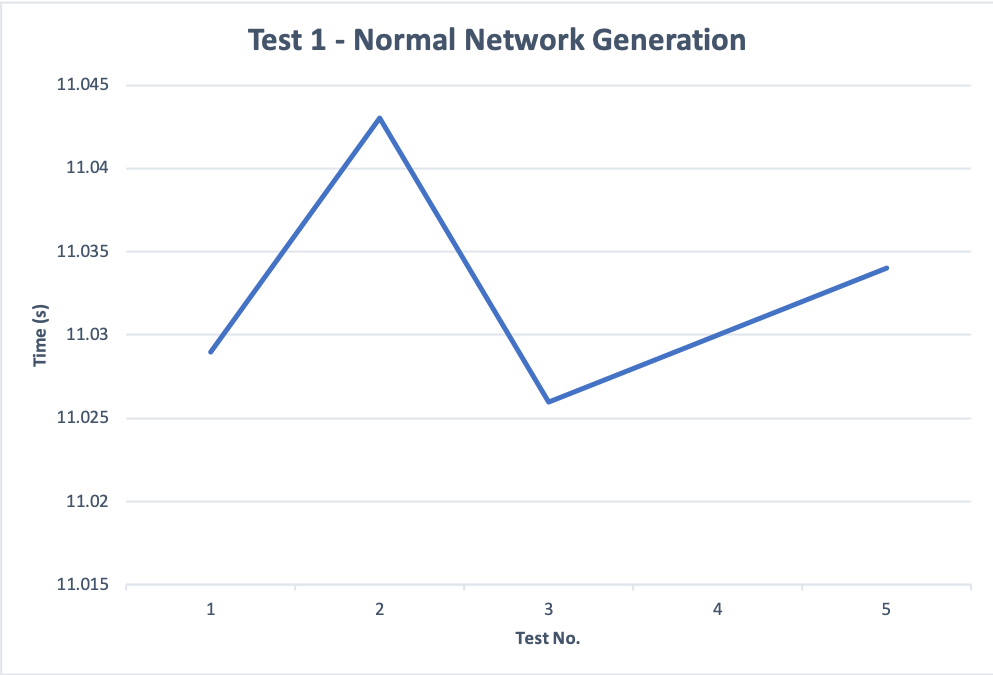
\includegraphics[scale = 0.4]{Images/Results/unittest1.png}
            \captionof{figure}{Graph of Unit Test 1}
             \label{fig:unittest1}
	\end{minipage}
\end{table}
As can be seen in the results from Table \ref{table:unittest1} the running time for generating 10 seconds worth of normal network data is, on average 11 seconds. As the web-traffic-generator is running for 10 seconds this means that collating the network packets and extracting the features from them takes approximately 1 second. The graph in Figure \ref{fig:unittest1} again shows that as the tests were completed the time taken remained consistent. This data generation will generate 10 rows of data in the dataset as the network packets are collated per second.
\subsection{Network Data Collection}
In extension to unit test 1, unit test 2 was built to test the amount of time required to collect network data and extract the required features from them. The test was run for differing times to see how increasing the amount of network data would alter the time taken to process it.
\begin{table}[H]
\centering
\caption{Results of Unit Test 2}
\label{table:unittest2}
\begin{tabular}{ccccc}
 \textbf{Generate Time (s)}&\textbf{Test 1 (s)}&\textbf{Test 2 (s)}&\textbf{Test 3 (s)}&\textbf{Average (s)}\\
 \hline
    1 & 2.067& 2.062& 2.045& 2.058\\
    10& 11.159& 11.203& 11.217& 11.193\\
    50& 52.165& 51.971& 51.691& 51.94233333\\
    100& 102.557& 102.782& 02.423& 102.5873333\\
    200& 206.891& 203.733& 204.192& 204.9386667\\
    600& 612.432& 614.682& 615.499& 614.2043333\\
\end{tabular}
\end{table}
\begin{figure}[H]
    \centering
    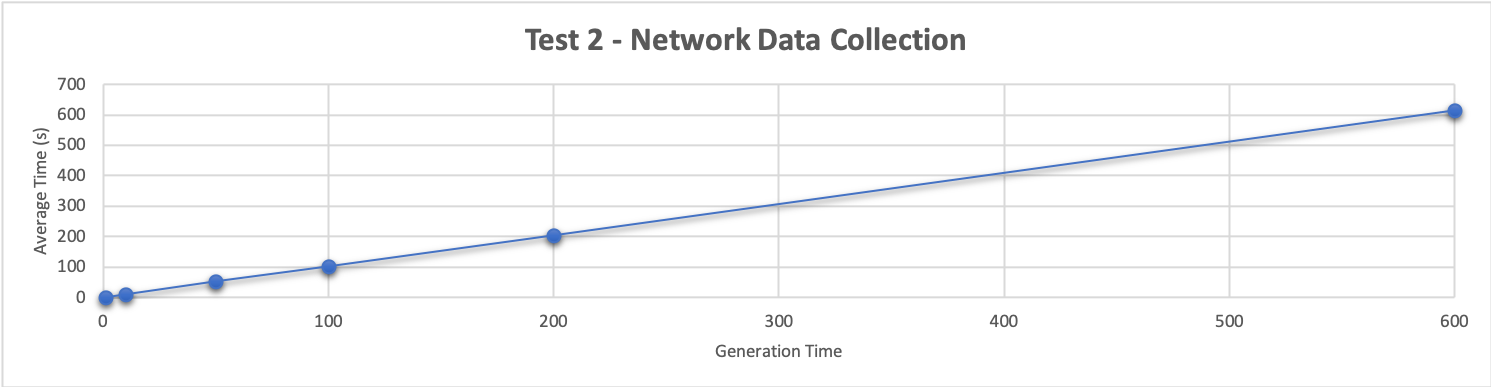
\includegraphics[scale = 0.5]{Images/Results/unittest2.png}
    \caption{Graph of Unit Test 2}
     \label{fig:unittest2}
\end{figure}
As can be seen by the results in Table \ref{table:unittest2} and the graph in Figure \ref{fig:unittest2}, as the time increases and the amount of network data increases, the time required to process the data also increases linearly. This makes sense as processing this data is done with pandas dataframe, which supports array programming where methods can be applied to a dataframe as a whole rather than to the individual features, which reduces time.

\subsection{Generating Attack Data}
The unit test for generating attack data will spin up two virtual machines and run a synflood attack for one minute before shutting down the machines, extracting the relevant features and removing all virtual machine files. The  \texttt{test\_attack\_generation()} function within the test file will execute this scenario.
\begin{table}[H]
\centering
\caption{Results of Unit Test 3}
\label{table:unittest3}
\begin{tabular}{cccc}
    \textbf{Test No.}& \textbf{Target (min)}&\textbf{Attack(min)}& \textbf{Full Scenario (min)}\\
    \hline
    1& 1:39	&2:39& 4:51\\
    2& 1:41	&2:43& 4:27\\
    3& 1:44	&2:49& 5:16\\
    4& 1:30	&2:17& 4:15\\
    5& 1:35	&2:10& 5:04\\
    \hline
    \textbf{Average} & 1:37 & 2:31& 4:46
\end{tabular}
\end{table}
As can be seen in the results from Table \ref{table:unittest3} the generation of the attack machine tended to take on average 1 minute 37 seconds while the target machine took, on average almost an extra minute to launch. This is in part due to the absence of a communicator or provisioner in the target machine, leaving packer to do less configuration. This was also due to the lower relative size of the target machine image in comparison to the attack machine. The target machine was 4.16GB while the attack machine was 10.85GB. 

The average execution time for the one minute data generation was 4 minutes 46 seconds. 2 minutes 30 were taken up on average launching the machine, about 30 seconds were taken for the attack machine to boot and a minute was taken for the attack leaving about 46 seconds the program took to power off machines and clear the virtual machines. 

Data generation in this form often resulted in less than the expected 60 rows of data. This is due to the fact that sometimes there are no packets to or from the target machine, especially before or after the attack runs and as such Scapy does not collect any packets. 

\subsection{Decision Tree Modeling}
This unit test was used to train the decision tree with the generated network data from the full system testing. The system will train five decision tree models and will run the relative metrics. A maximum depth of 5 was used during testing.
\begin{table}[H]
\centering
\caption{Results of Unit Test 4}
\label{table:unittest4}
\begin{tabular}{ccccc}
    \textbf{Test No.}&\textbf{Time (s)}& \textbf{Accuracy}& \textbf{Precision}&	\textbf{Recall}\\
    \hline
    1& 3.421& 99.8\%& 99.4\%& 99.3\%\\
    2& 3.697& 99.9\%& 99.7\%& 99.4\%\\			
    3& 4.081& 99.9\%& 99.9\%& 99.4\%\\
    4& 3.721& 99.9\%& 99.8\%& 99.9\%\\
    5& 3.856& 99.7\%& 99.7\%& 99.9\%\\
    \hline
    \textbf{Average} & 3.755& 99.8\%& 99.7\%& 99.3\%\\
\end{tabular}
\end{table}
As can be seen in Table \ref{table:unittest4} the decision trees modeled from the dataset which was generated during full system testing. The cross validation scores for each decision tree are seen below.
\begin{verbatim}
    Tree 1 - [0.99828263 0.99705594 0.99926398 0.9990184 0.99386503]
    Tree 2 - [0.99828263 0.9968106 0.99926398 0.9990184 0.99386503]			
    Tree 3 - [0.99828263 0.99705594 0.99926398 0.9990184 0.99386503]
    Tree 4 - [0.99828263 0.9968106 0.99901865 0.9990184 0.99386503]
    Tree 5 - [0.99803729 0.9968106 0.99901865 0.9990184 0.99263804]
\end{verbatim}
The decision trees have an accuracy and an average cross validation score  of 99\% which shows that the decision tree makes accurate decisions based solely on the data which has been generated by the user. It also shows that decision trees are a good classifier to use in this scenario. The decision tree also has a 99\% Recall and Precision which indicates that the decision tree has a low level of False negative and false positives which indicates that the generation of data through the virtual machines had no adverse effect to the modeling. On average the time taken to train the decision tree, test and extract the tree is just under four seconds. This is due to the dataset containing threats which are easily differentiated. 

\begin{figure}[H]
    \centering
    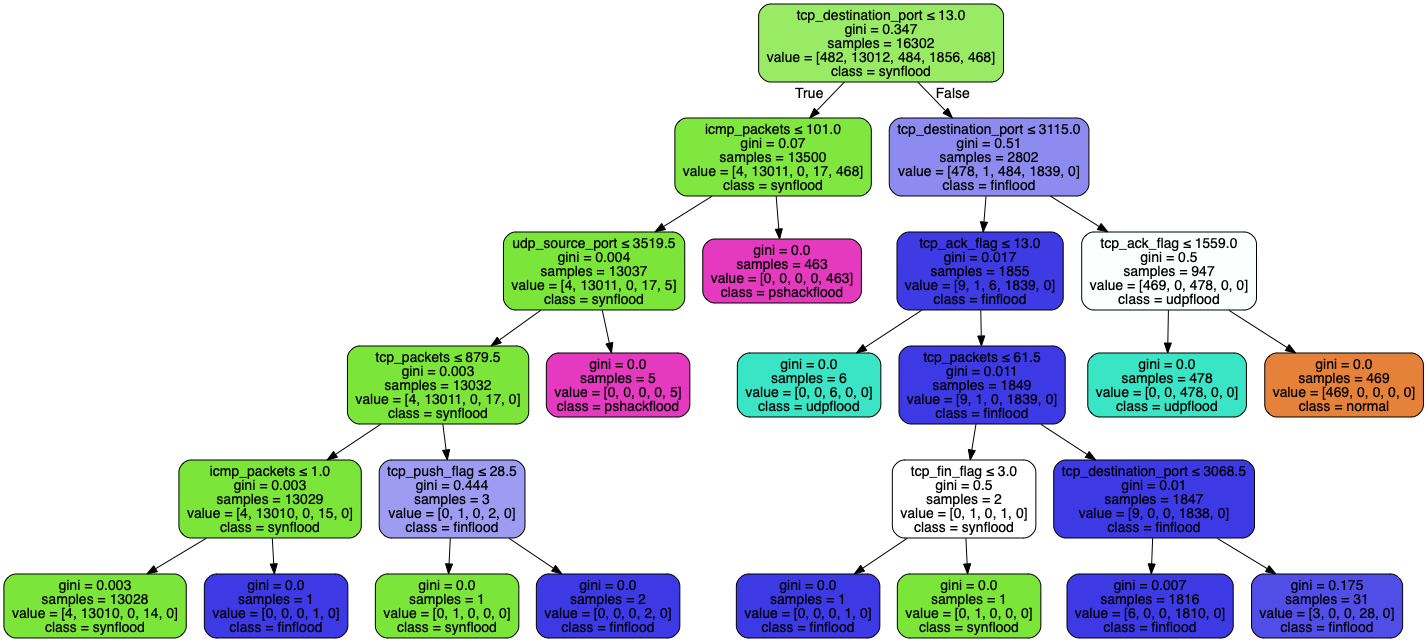
\includegraphics[scale=0.3]{Images/Results/tree.png}
    \caption{Decision Tree}
    \label{fig:dectres}
\end{figure}

The decision tree which was generated in the full system testing can be seen in Figure \ref{fig:dectres}. As can be seen the tree is relatively compact and as such can be considered to be not overfit. Overfitting can also be ruled out by looking at the metrics, which used cross validation and other methods to ensure the randomness of the test set. Therefore without defining a max\_depth the tree does not overfit the data despite certain sections of the tree in \ref{fig:dectres} containing nodes which define the same class.

The project was successful in generating a large scale dataset to be used within a decision tree model, however collating network data by the second means that the amount of data which is able to be generated is dependant on the time which the system can run for. For instance receiving 1 million rows of data for a particular attack will require the system to run for one million seconds which translates to just under 12 days. The workload can be reduced by running the program on multiple machines or by utilising different features. The project therefore is reliant on the amount of time which the user can spare, while 10 minutes seem appropriate for these attacks it may take longer if the differences between attacks are less clear.

The project only focuses on collecting network data from the machines, as detailed in the background section this is sufficient for threats such as DoS and Probe attacks but is not sufficient for R2L or U2R threats as these alter system files within the computer. The project does not collect any system logs at the moment but the collection of system logs can be automated in the target machine by using Packer provisioners.
\section{Requirement Based Testing}
Requirement based testing involves testing the created system based on the requirements set within Chapter \ref{chp:req}. All system requirements have been detailed below however not all other requirements have been detailed due to the subjective nature of a few of them.
    \begin{tabularx}{\textwidth}{|c|X|X|}
    \caption{Implemented Requirements}
    \label{table:irq}\\
    \hline
     \textbf{Code}& \textbf{Requirement Details}&\textbf{Implementation Details}\\
     \hline
     OS.1  & The system should automatically generate a virtualised network and simulate an attack & The system can generate two virtual machines from images and can run shell scripts on the attack machine to attack the target.\\
     \hline
     OS.2 & The system should collect the data from the simulated attack, the program should extract the relevant features and process the data into a dataset & The \texttt{data\_processing} package allows the user to both process raw network packets or process live network data from the \texttt{data\_generation} package. \\
     \hline
     OS.3 & The system should train a decision tree model to differentiate between different DoS attack & The user is able to specify the dataset when calling the \texttt{model} command. \\
     \hline
     OS.4 & The system should allow users to write their own attacks and to be able to run them in the virtual network & The user is able to specify the path and name of their attack when calling the \texttt{generate} command.\\
     \hline
     OS.5 & The system should allow the user to implement their own versions of each section to meet their requirements & The source code uses open source packages and so can be supplied on Github. The code is written in three separate packages which can be altered or and swapped.\\
     \hline
     DG.1 & The program must be able to automatically import 2 or more virtual machines from images, power on the virtual machines and run programs on each virtual machine. & The system can take two virtual machine images, specified in a config file, and generate two virtual machines from packer templates.\\
     \hline
     DG.2 & The virtual machines must connect to the same network and be accessible to both the host computer and each other & The images are set to connect to a bridged network and the packer template uses a vboxmanage command to ensure the interface is correct.\\
     \hline
     DG.3 & The virtual machines must power off after data collection is finished and they must delete themselves and their files. & The machines are powered off by Packer and the files removed either by the exit handler or the \texttt{clearvms} command. \\
     \hline
     DG.4 & The virtual machines must have the same IP address, they can be later identified from these IP address & This is set on each individual operating system.\\
     \hline
     DG.5 & The program must collect the network data which moves between the virtual machines & This was originally achieved by launching wireshark but is currently implemented by the \texttt{sniff()} function provided by the \texttt{scapy} library.  \\
     \hline
     DG.6 & The capture should run only when the attack starts and must stop when the attack finishes & The capture only starts when there is a response from the attack machine when pinged.\\
     \hline
     DG.7 & The program must also simulate normal network data and collect this data & The user is able to generate normal network data by running the web-traffic-generator using the \texttt{generate normal} command\\
     \hline
     DG.8 & The network packets must be saved to a file with a readable name & As wireshark is not used anymore the processed network data is now stored directly within the dataset. The path of the dataset is specified by the user. \\
     \hline
     DP.1 & The network packets need to be read from section \ref{sec:datagen}. & As the processing now occurs as soon as the network data comes in this is no longer necessary. However the previous implementation using \texttt{pyshark} is included. \\
     \hline
     DP.2 & The initial features, as in Table \ref{table:features_init} need to be extracted from the network data. & This is done by extracting the features from each packet and storing them within an array. \\
     \hline
     DP.3 & The packets need to be collated per second and the features, as in Table \ref{table:features}, need to be extracted & The packets are converted to a dataframe and then collated.\\
     \hline
     DP.4 & The packets need to be saved to a comma separated value (CSV) which will contain all the threats. & The generated dataframes are written to the csv path specified within the configuration file.\\
     \hline
     DM.1 & The model must be trained by data which was generated from the virtual machines & The user can specify the path when executing the \texttt{model} command\\
     \hline
     DM.2 & The model should be able to predict attacks with a >90\% accuracy. This is due to the KD99 dataset generating >90\% accuracy models \cite{SANGKATSANEE20112227} \cite{Peddabachigari} \cite{bouzida}. & This is achieved by the dataset the program was tested with.\\
     \hline
     DM.3 & The model should have a high amount of true positives and a small amount of false positives, a common issue in anomaly intrusion detection is a high level of false positives. & This is achieved by the dataset the program was tested with.\\
     \hline
     RE.1  & The project should run without error & This is achieved through good programming practice and testing.\\ 
     \hline
     RE.2 & Each section of the project should run without error independently & This is achieved in the project, each section is able to be run independently.\\
     \hline
     UP.1 & The program should be straightforward to use & The program uses sub commands and arguments in the command line, each command contains help screens and the config file is well commented. \\
     \hline
     UP.2 & The user should be able to use the system for their own uses without needing to understand how the code was implemented & The help screens and command line interface should allow usage of the program without extensive knowledge.\\
     \hline
     UP.3 & The project should not require special hardware to run, however may require a base spec to run sufficiently well. & 3GB of RAM and around 60GB of hard drive space is needed for the virtual machines to load. A dual core Intel i5 processor was used in testing however an i3 should be sufficent.\\
     \hline
     UP.4 & The process of data generation should be automated and should not require the user’s input & This has been achieved.\\
     \hline
     UP.5 & The project should run at a reasonable speed and not cause the system to crash & This was achieved on a 2017 Macbook pro with 8GB ram and a dual-core i5 processor.\\
     \hline
     UP.6  & The project should run on Windows, Mac and Unix Systems & The software has been tested on a Mac and an Ubuntu machine.\\
     \hline
\end{tabularx}
The project implemented all of the essential requirements and most of the important requirements and most desirable requirements were kept in mind and implemented in the project.
\subsection{Limitations}
The project has a few limitations due to the time spent on development or due to the scope of the project.
\begin{itemize}
    \item The project in its current state is only able to collect network data and does not collect any system logs
    \item The project only utilises two virtual machine images for a virtualised network as seen in Figure \ref{fig:vnd}.
    \item The system can take a long period of time to generate enough data for the user.
    \item The project does not aim to write any novel attacks. These must be written by the user if they require it.
\end{itemize}
\section{Project Evaluation}
The data generation section of the project provided the largest amount of issue, from designing to testing. The design was difficult due to my relative lack of understanding around the subject in the beginning. A large amount of time in the early times of the project were spent trying to fully understand the scope of this section and how it was to be implemented. Even when a design was fully realised, in practice changes were made to streamline the system as my knowledge of the area grew. The section as a whole works very well but took up a large chunk of time to develop, this was due to the time required to fully test a system. As can be seen from the results in this chapter a single one minute test can take up to five minutes, often when testing functionality which is due to happen after the machines close testing took several hours. This meant that this particular block took a much longer time than any other development block. Testing for the data generation block was done over the period of a few days due to the relatively small amount of attacks which had to be trained for. The smaller amount of threats and the relatively large amount of packets generated, by nature of the DoS attack, meant that the testing was rather straightforward. But as the attacks get more complex and more data is required then more time will be taken to generated enough data.

The data processing of the project was originally developed without issue, simply taking the data which had been generated previously and extracting the relevant features from it. However after much thought this was changed to allow it to be Incorporated with the data generation module. This reduced the time required to generate data and made a lot more sense. The design developed due to an increased experience with network data extraction modules in python allowing me to develop the packet sniffer in the program rather than using another third party piece of software which the user needs to install. The collection and processing of network data is fast, often taking around fourteen seconds to collate ten minutes of packet data. Testing involved simply running the code for different lengths of time to understand how the length of time taken to collect and extract data changed as the length of time data was required for changed also. Using an open source library allows the user to alter the features which they extract to better suit their needs.

The data modeling section of the project was developed with little issue. The section utilised the \texttt{sklearn} package to both implement the project and test it. The library had a large range of functions and modules to use during the implementation of the project. The library which allowed the development of this section to be completed and tested quickly. The models which were generated during testing had high accuracy and precision meaning that they could be utilised as very efficient intrusion detection systems, though the development of such intrusion detection system is beyond the scope of the project. 

The overall system was developed after the three sections above were completed. This me to ensure that the essential sections of the project worked and were developed properly before tying the sections together. Originally as these modules were separate packages they were imported into files much like libraries and their functions called when needed. However this did not make much sense as the functions rarely return anything and the user would have to develop a program to call and run the functions. Due to this the command line interface was developed in the hopes that the project would become more usable. The command line interface utilises simple syntax to allow the user to easily navigate the project. The sub commands are fairly self explanatory and the help pages indicate to the user exactly how they should use the sub-commands. A setup.py file was also written to ensure that the user can easily install dependencies.

Scheduling the development of the project was highly dependant on results from testing. The project could not continue until data had been generated for instance. This often meant than sometimes the time needed to develop a module was underestimated. While suitable time was found to develop the project more time should have been allocated to the blocks so as to ensure they were finished before moving on.

The agile software development methodology allowed me to develop the project in a much better way. When the project had started developing the ideas which now form a crucial part of the project such as the network collection or command line interface were not originally part of the design. The agile methodology allowed me to learn from development and return to previously designed sections of the project and alter them. Overall the project successfully created a model from a dataset formed of generated network data from an automated virtualised network.



